%%%%%%%%%%%%%%%%%%%%%%%%%%%%%%%%%%%%%%%%%%%%%%%%%%%%%%%%%%%%%%%%%%%%%%%%
% Plantilla TFG/TFM
% Escuela Politécnica Superior de la Universidad de Alicante
% Realizado por: Jose Manuel Requena Plens
% Contacto: info@jmrplens.com / Telegram:@jmrplens
%%%%%%%%%%%%%%%%%%%%%%%%%%%%%%%%%%%%%%%%%%%%%%%%%%%%%%%%%%%%%%%%%%%%%%%%

\chapter{State of Art}
\label{marcoteorico}
\textit{As we previously stated, semantic segmentation is a extremely important task in the field of computer vision due to its enormous value towards complete scene understanding. This chapter is organized as follows: Section \ref{sec:intro} will give a brief introduction to the Semantic segmentation problem. In section \ref{sec:sim2real} we will delineate the importance of the Sim To Real field, as well as review some of the latest works on the matter. In Section \ref{sec:architectures} we cover several of the most important and recent deep network architectures. Finally in Section \ref{sec:datasets} we take a look at some of the most important data-sets and frameworks that tackle the semantic segmentation problem. }

\section{Introduction}
\label{sec:intro}
Before we dive into the next sections it is important to understand the semantic segmentation problem and where it comes from. Semantic segmentation is a natural evolution of the object recognition problem, the goal is to infer the class for every pixel on the image, obtaining a pixel-by-pixel labeled output. 
Semantic segmentation is not so different from classic object recognition, in fact it is fundamentally the same, it just adds an extra layer of complexity towards a more fine-grained solution. We could go further and try to differentiate instances of the same class, that would be instance segmentation, Figure \ref{fig:object_recognition} shows the different object recognition solutions from less to more complex.

\begin{figure} [h]
	\centering
	\begin{tabular}{cccc}
		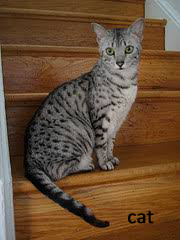
\includegraphics[width=0.223\textwidth]{archivos/cat_classification.png} &
		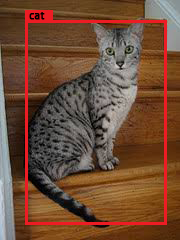
\includegraphics[width=0.223\textwidth]{archivos/cat_localization.png} &
		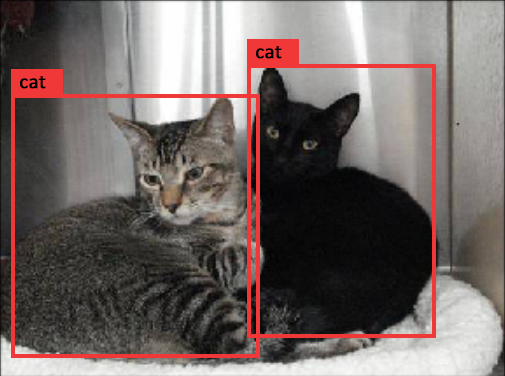
\includegraphics[width=0.4\textwidth]{archivos/cats_localization.png} \\
		\textbf{(a)}  & \textbf{(b)} & \textbf{(c)}  \\[6pt]
	\end{tabular}
	\begin{tabular}{cccc}
		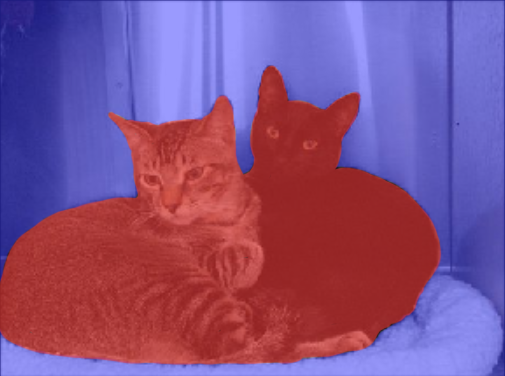
\includegraphics[width=0.4\textwidth]{archivos/cats_semantic_segmentation.png} &
		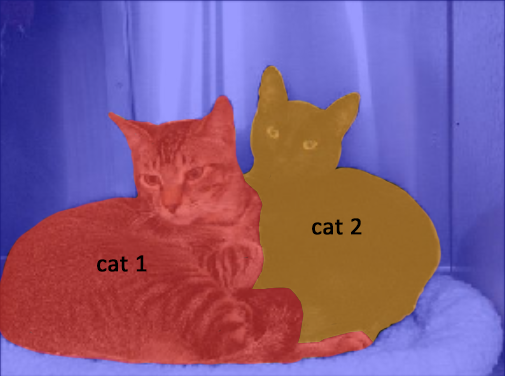
\includegraphics[width=0.4\textwidth]{archivos/cats_instance_segmentation.png} \\
		\textbf{(d)}  & \textbf{(e)}  \\[6pt]
	\end{tabular}
	\caption{ \textbf{(a)} Object detection
		\textbf{(b)} Object localization
		\textbf{(c)} Multiple object localization
		\textbf{(a)} Semantic segmentation
		\textbf{(b)} Instance segmentation.}
	\label{fig:object_recognition}
\end{figure}

\section{Sim 2 Real}
\label{sec:sim2real}
In the last decade, data driven algorithms have vastly surpassed traditional techniques for computer vision problems, these algorithms, although can be tuned and improved in many different ways, still require vast amounts of quality, precisely annotated data in order to yield good results. In the real world environment, there are quite a few limitations to the quantity and quality of the data that can be produced. For instance, we could be limited to the number of cameras and annotators, moving physical objects to setup scenes could also be difficult and time consuming, and dangerous situations could be risky to set up properly i.e trying to get an autonomous car to learn to avoid pedestrians when there is no time to brake.
    
Sim2Real is a specific section of the data science field that mainly focuses on the automatic generation and ground-truth annotation of synthetic data by simulating the real world in a virtual environment. Although a virtual environment will allow us to workaround the previously mentioned restrictions, there's still a reality gap that must be covered in order for the synthetic data to be transferred to real life situations. Most synthetic data scenarios will present discrepancies between them and the real world, to overcome this and properly transfer the knowledge to real problems there are two known approaches that have been proven to be effective: 

\begin{itemize}
	\item \textbf{Photorealism:} This is the most intuitive approach and the main idea behind it is to simply generate extremely realistic environments as close to reality as possible, to achieve this multiple techniques can be applied and the current state of the art in this field has grown substantially in the last decade. Such techniques include rendering very high and photo-realistic textures, models and lightning or simulating the noise of real cameras by applying filters and post-process effects. 
	
	One of the most recent and promising innovation is real time Ray Tracing, which is a technique that substitutes the traditional rasterization step of the classic rendering pipeline, Figure \ref{fig:pipeline} illustrates both pipelines. Instead of discretizing the scene and assigning the pixel values, Ray Tracing simulates the behavior of the lightning by casting (tracing) the path of light as pixels, simulating effects such as reflection, refraction and scattering. This allows for higher precision in the pixel values since it takes into account all of the materials of the scene where the light bounced.
	
	\begin{figure}
		\centering
		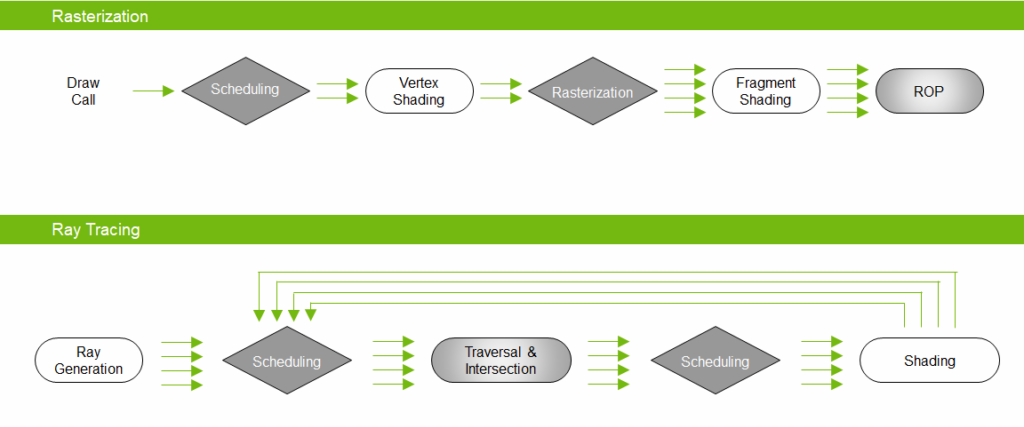
\includegraphics[width=\linewidth]{archivos/pipeline}
		\caption[Traditional rasterization pipeline in contrast to the Ray Tracing pipeline.]{Traditional rasterization pipeline in contrast to the Ray Tracing pipeline. Extracted from NVIDIA devblog\footnotemark.}
		\label{fig:pipeline}
	\end{figure}
	\footnotetext{\url{https://devblogs.nvidia.com/vulkan-raytracing}}
	
	Normally, Ray-Tracing techniques are performed offline since they are quite heavy in terms of computation times. However, the recent RTX NVIDIA Graphic cards \footnote{\url{https://www.nvidia.com/es-es/geforce/20-series/}} feature a new type of processing unit, the RT cores, which specialize in Ray-Tracing computing and are able to accelerate such process, allowing for real time Ray-Tracing. Although this technique is still relatively recent, it is very promising and worth keeping an eye on it.

	\item \textbf{Domain randomization:} This is the main alternative to photorealism when trying to cover the reality gap between the real world and the synthetic environments. This technique is based on showing the model a large amount of randomized variations of certain synthetic object or environment, this is done by randomizing certain inputs like the materials, lightning, animations or meshes. With this method even if the data is not represented with extreme fidelity, the variability of the multiple range of slightly different samples will make up for it, with enough randomization, the real world will appear as just another variation which will allow the model to generalize. Figure \ref{fig:domainrandomization} shows an example of randomized training inputs.
	
	\begin{figure}
		\centering
		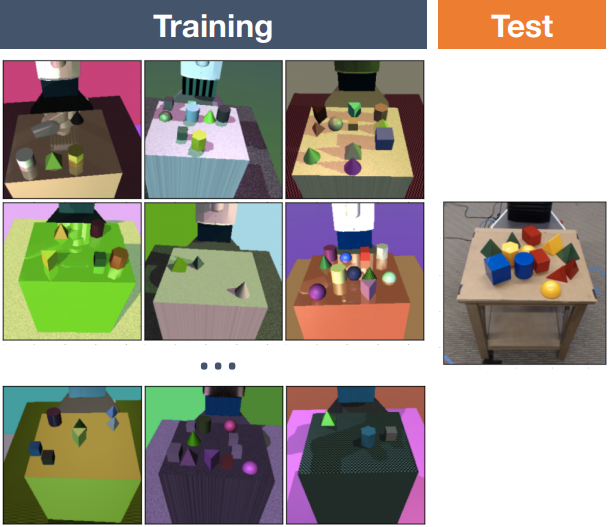
\includegraphics[width=0.5\linewidth]{archivos/domain_randomization}
		\caption{Low-fidelity images with random variations in camera angle, lightning and positions are used to train an object detector. Testing is done in the real world. Image from \cite{DBLP:journals/corr/TobinFRSZA17}.}
		\label{fig:domainrandomization}
	\end{figure}

	Another interesting approach to reduce the reality gap was researched in a 2018 paper by \cite{DBLP:journals/corr/abs-1812-05040}. In this work they present \textbf{Domain Adaptation}, the main takeaway behind this idea is to transfer the real-world style of images into the synthetic ones. This is done by a \gls{gan}, the image transform network generates an image taking the synthetic RGB image, the segmentation masks of said image, as well as the depth map. The discriminator will have to differentiate between the real image and the one generated by the network. 
	
	Also a second adaptation pass is done at the output level. The Task Network is the responsible for predicting the outputs of both real and synthetic images. Then it goes through another discriminator which has to discern if the outputs are predicted from a real or the synthetic adapted image. Figure \ref{fig:gan} shows their proposed architecture.
	
	\begin{figure}
		\centering
		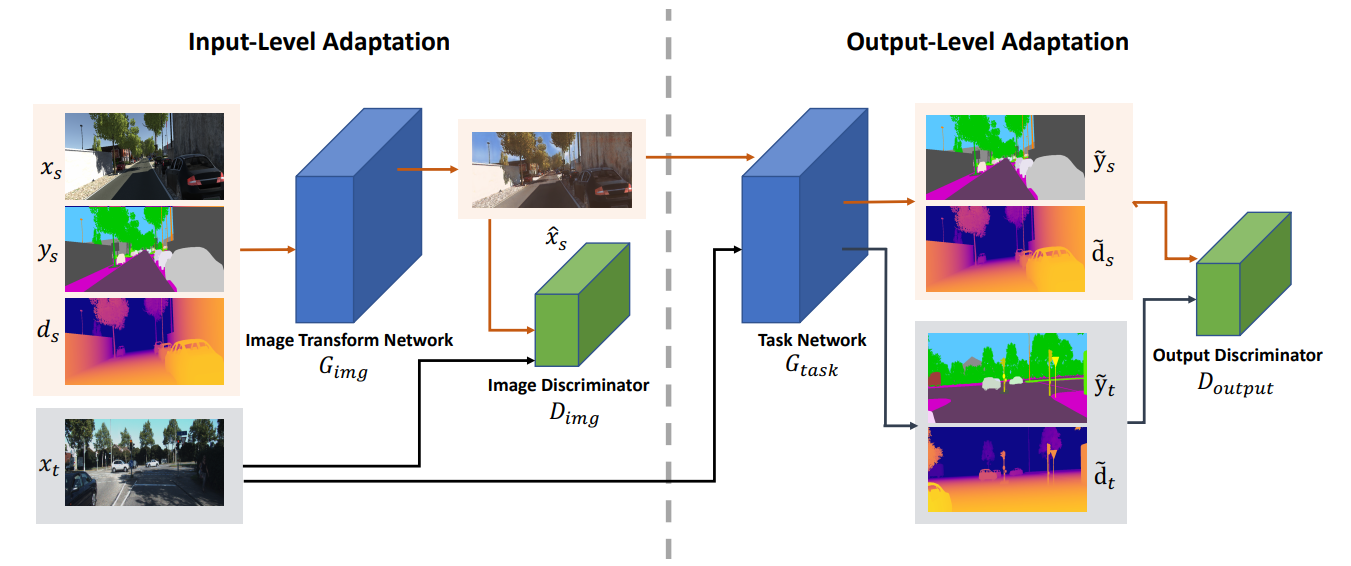
\includegraphics[width=\linewidth]{archivos/gan}
		\caption{Overview of the Input-Output adaptation network form \cite{DBLP:journals/corr/abs-1812-05040}}
		\label{fig:gan}
	\end{figure}
 
\end{itemize}

\subsection{VirtualHome}
VirtualHome is a three dimensional environment built in the Unity game engine. The main goal is to model complex tasks in a household environment as sequences of more atomic and simple instructions.
 
In order to perform this task a big database describing activities composed by multiple atomic steps was necessary, in the human natural language there is a lot of information that is common knowledge and is usually omitted, however, for a robot or agent this information has to be provided in order to fully understand a task. For this purpose an interface to formalize this tasks was built on top of the Scratch \footnote{\url{https://scratch.mit.edu/}} MIT project. Then all of this atomic actions and interactions were implemented using the Unity3D game engine.

For the data collection, they had workers describe in natural language all of these tasks and then built them using the Scratch interface. Every task is composed by a sequence of steps where every step is a Scratch block, and every block defines a syntactic frame and a list of arguments for the different interactions that they may have.

Every step $t$ in the program can be written as:

\[ step_t = [action_t] (object_{t,1})(id_{t,1}) ... (object_{t,n})(id_{t,n}) \]

Where $id$ is an identifier to differentiate instances of the same object. An example program to "watch tv" would look like this: 
\newline

$step_1$ = [Walk] (TELEVISION)(1)

$step_2$ = [SwitchOn] (TELEVISION)(1)

$step_3$ = [Walk] (SOFA)(1)

$step_4$ = [Sit] (SOFA)(1)

$step_5$ = [Watch] (TELEVISION)(1) \newline

Another example this time with the scratch block interface can be seen in figure \ref{fig:virtualhome_example}.

\begin{figure}[h]
	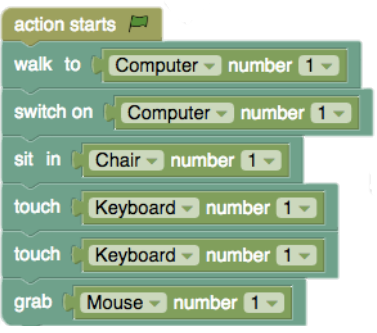
\includegraphics[scale=0.5]{archivos/virtualhome_example.png}
	\centering
	\caption{List of actions represented with the scratch interface, where the user can manually add, modify and change the arguments of every action.}
	\label{fig:virtualhome_example}
\end{figure}

\subsection{UnrealROX}
UnrealROX \cite{DBLP:journals/corr/abs-1810-06936} is a photo-realistic 3D virtual environment built in \gls{ue4} capable of generating synthetic, ground-truth annotated data. Unlike VirtualHome, the main method to record sequences is to actually control the actors manually making use of the \gls{vr} headset and controllers, this will be further explained in the following chapters.

\section{Common Architectures}
\label{sec:architectures}
As we previously stated, semantic segmentation is a natural step towards the more fine-grained image recognition problem, since the information that we are trying to infer is higher level, we will also require more complex architectures. Although the models we will be reviewing in this section work properly for image recognition and detection, some modifications will have to be made in order to adapt them for segmentation problems. However, they have made such significant contributions to the field that they are still being used as the basic building blocks of segmentation architectures.

\subsection{AlexNet}
AlexNet was the first deep network architecture that successfully surpassed traditional machine learning approaches, winning the \gls{ilsvrc} 2012 with a 84.6\% TOP-5 test accuracy, easily surpassing the its competitors by a huge margin. The architecture itself was pretty straight forward. It consisted of five convolution + pooling layers followed by three fully connected ones as seen in figure \ref{alexnet}.

\begin{figure}[h]
	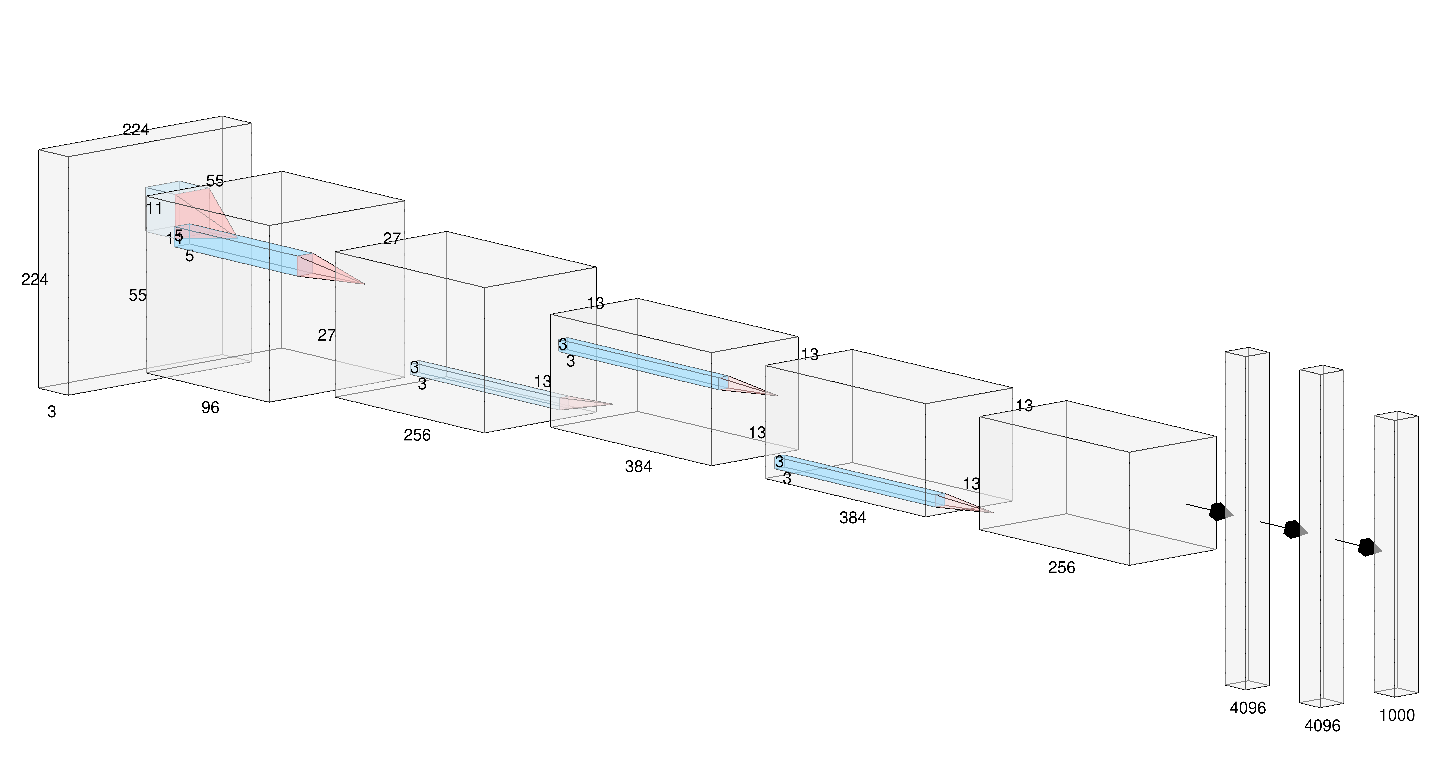
\includegraphics[scale=0.3]{archivos/alexnet.png}
	\centering
	\caption{AlexNet architecture reproduced from \cite{AlexNet}}
	\label{alexnet}
\end{figure}

\subsection{VGG}
VGG (\cite{DBLP:journals/corr/SimonyanZ14a}) is also a deep network model introduced by the \gls{vgg}, one of the various model configurations proposed was submitted to the \gls{ilsvrc} 2013. The VGG-16 achieved 92.7\% TOP-5 test accuracy.

The structure of VGG-16 is also quite simple and not too deep, as its own name hints, it consists of 16 convolutional layers, and just like AlexNet, uses three fully connected layers for classification. The main improvement over AlexNet was made substituting the first large kernel sizes in the first few layers with multiple 3x3 sequential kernel filters.

\subsection{GoogLeNet}
GoogLeNet (also known as Inception) was introduced by (cite) and was submitted to \gls{ilsvrc} 2014, winning with a TOP-5 test accuracy of 93.3\%. GoogLeNet architecture is rather complex, it introduced the inception module (shown in Figure \ref{inception}) which consisted of a new approach where convolution layers were not stacked in just sequential order but instead had some of them compute in parallel, which substantially reduced computational cost. The outputs of the different layers where then concatenated and moved towards the next module.

\begin{figure}
	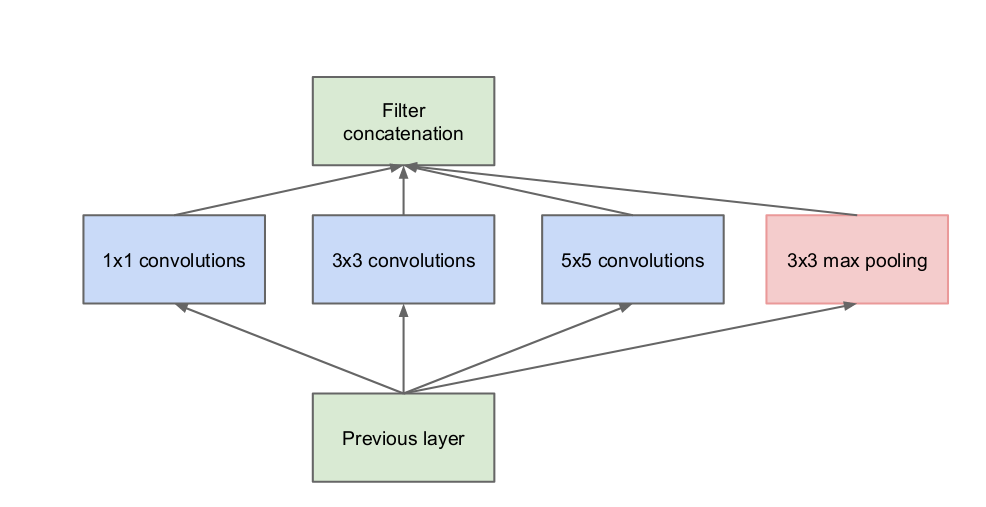
\includegraphics[scale=0.3]{archivos/inception_module.png}
	\centering
	\caption{Inception module extracted from \cite{DBLP:journals/corr/SzegedyLJSRAEVR14}}
	\label{inception}
\end{figure}

Ever since their first version Inception v1, they have been constantly releasing new iterations of the network with constant performance improvements, up to their last Inception v4 release.

\subsection{ResNet}
ResNet \cite{DBLP:journals/corr/HeZRS15} was first introduced by Microsoft research and it got very popular after achieving 96.4\% in \gls{ilsvrc} 2016. This \gls{cnn} is extremely deep with 152 layers (although shallower variations do exist) and it introduced a new concept called residual blocks. Since AlexNet was released, \gls{cnn} have become increasingly deeper, this makes the network more prone to the vanishing gradient problem (the backpropagated gradients gets infinitely small and the network performance falls off). The new residual module allowed the network inputs to skip layers and copy the values onto deeper layers, in a way that the compute output is a combination of $X$ and $F(X)$ as depicted in Figure \ref{fig:residual}. This helps reducing the vanishing gradient problem in deep networks and allows each layer with a residual input to learn something new since the inputs are both the encoded values from the previous layer as well as the unchanged inputs.

\begin{figure}
	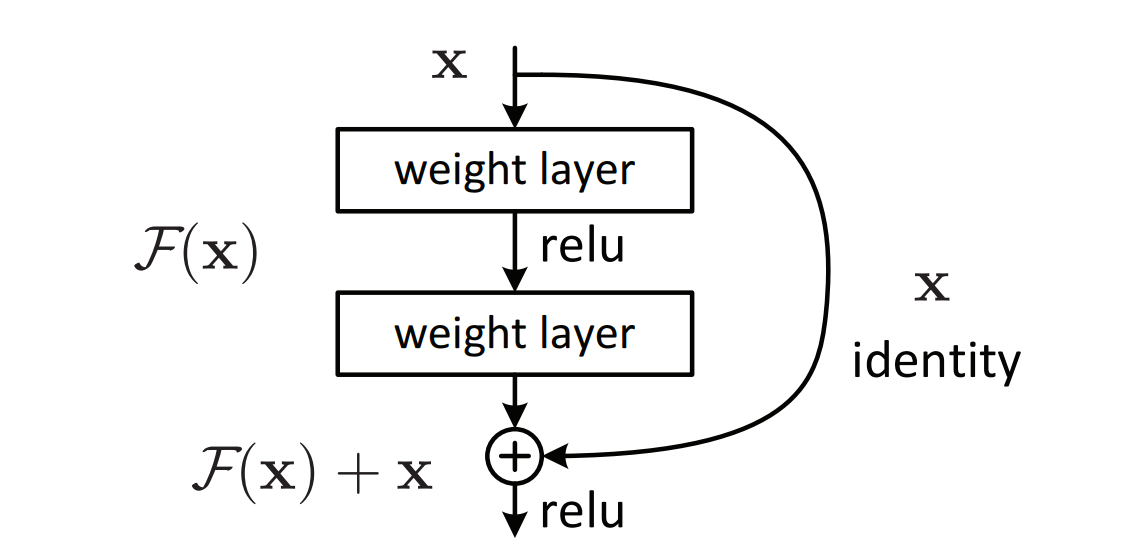
\includegraphics[width=0.5\textwidth]{archivos/residual.png}
	\centering
	\caption{Residual block extracted from \cite{DBLP:journals/corr/HeZRS15}}
	\label{fig:residual}
\end{figure}

\subsection{ReNet}
Multi Dimensional Recurrent Neural Network (MDRNN) are a variation of regular RNN that allow them to work with $d$ spatio-temporal dimensions of the data. The architecture proposed by (cite) used regular RNN instead of MDRNN, where every convolution + pooling layer is replaced by four RNN's that sweep the image across in four directions. 

\subsection{Semantic Segmentation Methods}
All the image recognition problem solutions based on convolutional architectures, whether it is recognition, detection, localization or segmentation, they all share a big common module, which is the convolution layers that will extract the features of any image, then the feature maps can be applied to any classification network structure depending on the desired output format.

Today, almost every semantic segmentation architecture uses the \gls{fcn} by \cite{DBLP:journals/corr/LongSD14}. The idea behind this is to replace the classic fully connected layers of \gls{cnn}s with \gls{fcn}s in order to obtain a spatial map instead of classification outputs, this way we can obtain pixel-wise classification while still using the inferred knowledge and power of the \gls{cnn}s to extract the features. However, a new problem arises when using \gls{cnn}s for semantic segmentation since  convolutional layers (convolution + pooling) downsample the input image in order to learn features, this downsampling does not matter when applied to classification problems, however, when doing pixel-wise classification, we require the output image to have the same size as the input. To overcome this problem, spatial maps are then upsampled by using deconvolution layers as shown in \cite{deconvolution}.

\subsubsection{Decoder Variant}
The decoder variant is another method to adapt networks that were initially made for classification. In this variant, the network after removing the fully connected layers is normally called encoder and it outputs a low-resolution feature map. The second part of this variant is called decoder and the main idea behind it is to up-sample those feature maps to obtain a full resolution pixel-wise classification.

One of the most known examples of this encoder-decoder architecture is SegNet \cite{DBLP:journals/corr/BadrinarayananK15}, the encoder part is fundamentally the same as a \gls{vgg}-16 without the fully connected layers at the very end, while the decoder part consists of a combination of convolution and upsampling layers that correspond to the max-pooling ones in the encoder, the whole architecture can be seen in figure \ref{fig:segnet}. SegNet is a very simple architecture which yields very good results and is relatively fast, which makes it a good starting point of any semantic segmentation problem.

\begin{figure}[h]
	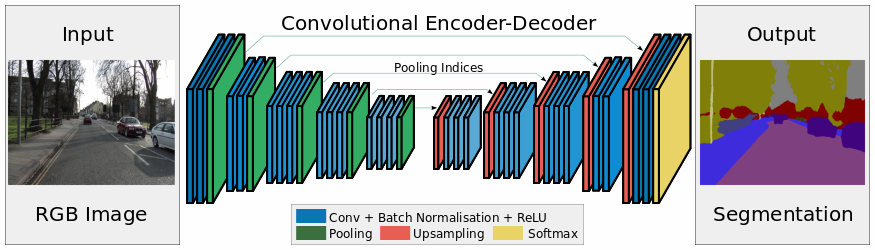
\includegraphics[scale=0.5]{archivos/segnet.png}
	\centering
	\caption{Segnet architecture graph extracted from \cite{DBLP:journals/corr/BadrinarayananK15}}
	\label{fig:segnet}
\end{figure}

\subsubsection{Dilated Convolutions}
As we previously mentioned, \gls{cnn}'s generate significantly reduced spacial feature maps, to overcome this spatial reduction, dilated convolutions (also known as \textit{atrous} convolutions) can be used in order to aggregate multi-scale contextual information without down-scaling.

The dilation rate $l$ will control the up-sampling factor of the filters. That way, a 1-dilated convolution would be a regular convolution where every element has a receptive field of 1x1, in a 2-dilated every element has a 3x3 receptive field, in a 3-dilated every element has a 7x7, this is depicted in Figure \ref{fig:dilatedconv}. This way the receptive field grows in a exponential way, while the parameters have a linear growth.

\begin{figure}
	\centering
	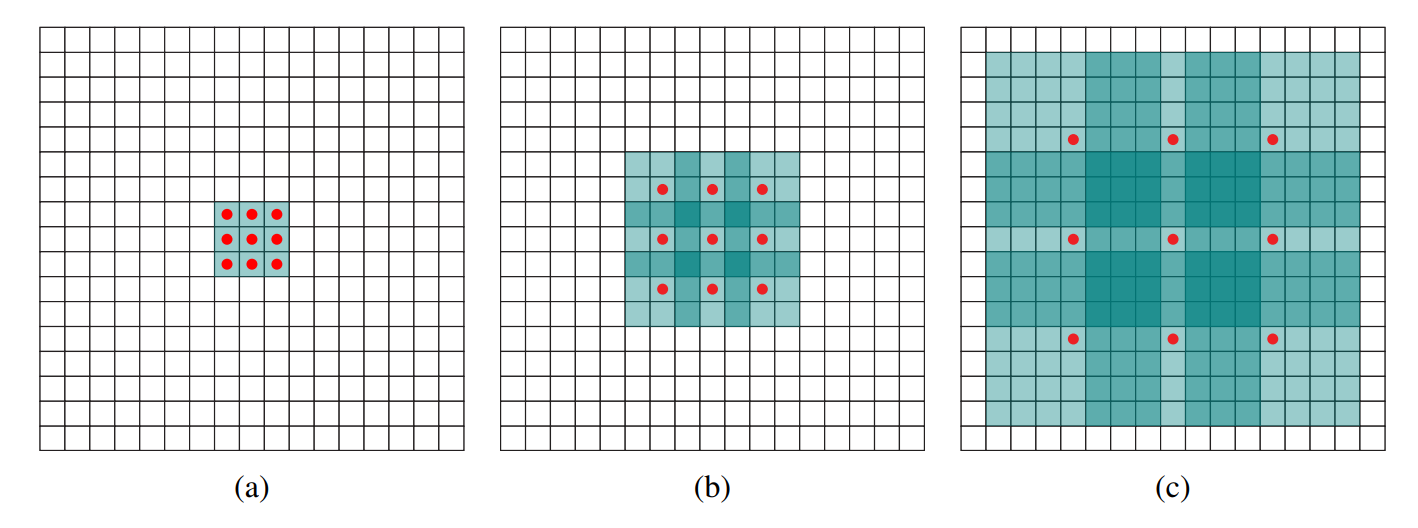
\includegraphics[width=0.7\linewidth]{archivos/dilated_conv}
	\caption{(a) 1x1 receptive fields, 1-dilated, (b) 3x3 receptive fields, 2-dilated, (c) 7x7 receptive fields, 3-dilated. Figure extracted from \cite{yu2015multiscale}.}
	\label{fig:dilatedconv}
\end{figure}

Some of the most important works that make use of this technique are the aforementioned multi-context aggregation by \cite{yu2015multiscale} and DeepLab by \cite{DBLP:journals/corr/ChenPK0Y16}.

\subsubsection{Conditional Random Fields}
Deep \gls{cnn}s applied to semantic segmentation excel at classification tasks, however they still lack precision when it comes to spacial information and struggle to properly delineate the boundaries of objects. To overcome this, a last post-processing step in order to refine the output can be applied, for instance, \gls{crf}. \gls{crf}s make use of both low level pixel interaction as well as the multi-class inference pixel prediction of high level models.

The DeepLab model by \cite{DBLP:journals/corr/ChenPK0Y16} makes use of \gls{crf} to refine their output, an overview of the model can be seen in Figure \ref{fig:deeplab}. 

\begin{figure}
	\centering
	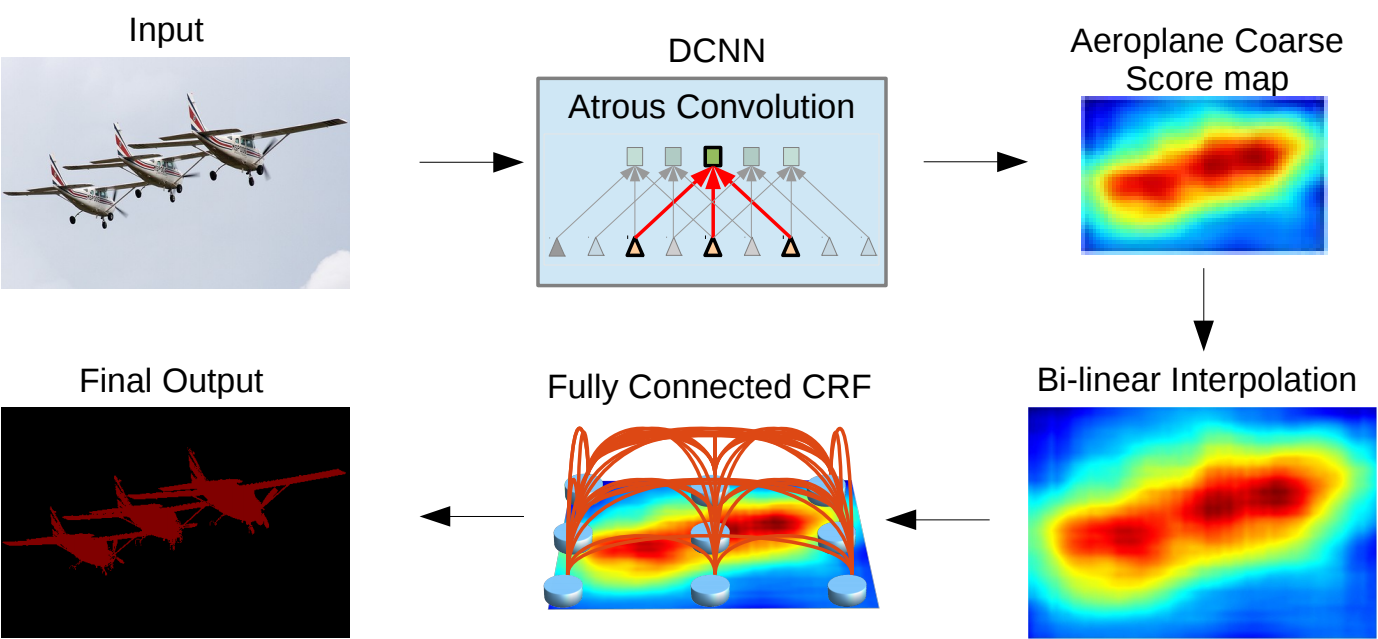
\includegraphics[width=0.7\linewidth]{archivos/deeplab}
	\caption{Illustration of the DeepLab proposed architecture, using a deep \gls{cnn} for pixel-wise classification and a fully connected \gls{crf} to refine the output.}
	\label{fig:deeplab}
\end{figure}

\section{Datasets}
\label{sec:datasets}
In this section we will review some of the most important datasets that are commonly used to train semantic segmentation architectures. 

\subsection{PASCAL}
PASCAL Visual Object Classes is one of the most popular 2D datasets for semantic segmentation. The challenge consists of 5 different competitions, 21 ground-truth annotated classes and a private test set to verify the accuracy of submitted models. Also there are a few extensions of this dataset such as PASCAL Context which provides pixel-level classification for the entire original dataset classes although only 59 of them are usually taken into account when working with classification problems since the rest of them are too rare, so they are normally considered as background. Another extension for the PASCAL dataset that is worth mentioning is PASCAL Part, which further decomposes the instances in smaller classes, for instance a car could be decomposed into wheels, chassis, headlights and windows, figure \ref{fig:pascal_part} shows more examples of different classes.

\begin{figure}[h]
	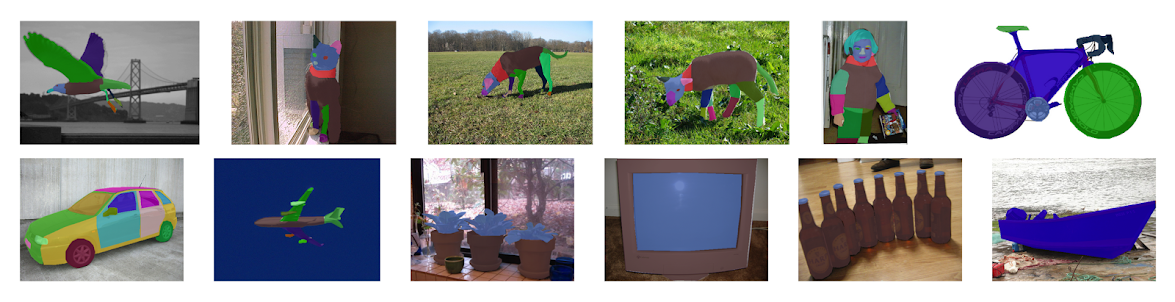
\includegraphics[scale=0.35]{archivos/pascal_part.png}
	\centering
	\caption{PASCAL Part examples of ground truth annotated parts for different classes.}
	\label{fig:pascal_part}
\end{figure}

\subsection{Semantic Boundaries Dataset}
This dataset is an extension of the PASCAL dataset that provides semantic segmentation ground-truth annotations for all the images that were not labeled in the original dataset. SBD greatly increases the amount of data from the original PASCAL and because of this is commonly used for deep learning architectures.

\subsection{Cityscapes}
Cityscapes is a urban dataset mainly used for instance and semantic segmentation. It contains over 25000 images and 30 different classes was recorded in 50 cities during different times of the day and year.

\subsection{KITTI}
The KITTI dataset \cite{Geiger2013IJRR} was recorded from a vehicle on a urban environment. It includes camera RGB images, laser scans, and precise GPS measurements. Despite being very popular for autonomous driving, it does not contain ground-truth annotations for semantic segmentation. To work around this, some researchers manually annotated parts of the dataset to fit their necessities. 

\subsection{COCO}
COCO is yet another image recognition and segmentation dataset by \cite{DBLP:journals/corr/LinMBHPRDZ14} which mainly focuses on everyday scenes and common objects. The dataset contains 91 different classes and a total of 328.000 images and the labeling methods contain both bounding boxes as well as semantic segmentation.